\documentclass[11pt,a4paper]{article}

\usepackage[T1]{fontenc}
\usepackage[utf8]{inputenc}
\usepackage[italian]{babel}
\usepackage{amsmath,amssymb}
\usepackage[a4paper,margin=2.5cm]{geometry}
\usepackage{array}
\usepackage{siunitx}
\usepackage{booktabs}
\usepackage{graphicx}
\usepackage{float}
\usepackage{hyperref}

\hypersetup{hidelinks}
\setlength{\parindent}{0pt}
\setlength{\parskip}{4pt}
\allowdisplaybreaks
\graphicspath{{figure/}}
\sisetup{output-decimal-marker={,}, group-separator={\,}, per-mode=symbol,
         exponent-product=\cdot, range-phrase={\text{--}}}

\newcommand{\uma}{u-a}
\newcommand{\upa}{u+a}
\newcommand{\Mr}{M_{r}}
\newcommand{\Ms}{M_{s}}

\title{Gasdinamica -- Svolgimento B65-E01\\[2pt]
\large Dati iniziali isentropici: espansione centrata, compressione centrata e soluzione asintotica}
\author{}
\date{Prova del 14/09/2021 -- Esercizio 1}

\begin{document}
\maketitle

\section*{Traccia}
Calcolare la soluzione per $t\ge0$ del problema monodimensionale non stazionario definito dalle condizioni
iniziali isentropiche
\begin{center}
\begin{tabular}{lll}
$x\le0$: & $0\le x\le1$: & $x\ge1$: \\
$p=1$, $u=0$, $a=\num{1.522}$ & $u=\num{2.61}-\num{1.856}\,x$, $a=1+\num{0.4995}\,x$ &
$u=\num{0.754}$, $a=\num{1.4995}$
\end{tabular}
\end{center}
Graficare la distribuzione della pressione e del numero di Mach in funzione di $x$ all'istante
$t=\num{0.4246}+\varepsilon$. Fornire una stima della soluzione asintotica. Riportare la soluzione sui piani
$x$--$t$ e $p$--$u$.

%==============================================================================
\section{Lettura del testo e dati}
I dati sono adimensionali. Il gas non è indicato: assumo $\gamma=\num{1.4}$, $\delta=(\gamma-1)/2=\num{0.2}$.
Non è una scelta arbitraria: è l'unico valore per cui $a+\delta u$ ha lo stesso valore ai due lati della
discontinuità in $x=0$, cioè per cui il salto iniziale è un'onda semplice; con un altro $\gamma$ in $x=0$
nascerebbero tre onde, e il dato $a=\num{1.522}$ sarebbe casuale.

``Condizioni iniziali isentropiche'' lo leggo come \textbf{entropia uniforme} (omoentropico): la pressione è
assegnata solo a sinistra e altrove segue da $a$ con l'isentropica.

Il profilo è continuo in $x=1$ (a $x=1$ la legge lineare dà proprio $u=\num{0.754}$, $a=\num{1.4995}$), mentre
in $x=0$ $u$ e $a$ saltano. Nomino gli stati iniziali:
\begin{table}[H]
  \centering
  \begin{tabular}{llll}
    \toprule
    Stato & Dove & $u$ & $a$ \\
    \midrule
    1 & $x\le0$ & 0 & \num{1.522} \\
    2 & $x=0^+$ (inizio del tratto lineare) & \num{2.61} & 1 \\
    4 & $x\ge1$ & \num{0.754} & \num{1.4995} \\
    \bottomrule
  \end{tabular}
  \caption{Stati iniziali; $p_1=1$, $\gamma=\num{1.4}$ (ipotesi).}
\end{table}
Si chiedono: la soluzione per $t\ge0$, i profili $p(x)$ e $M(x)$ a $t^*=\num{0.4246}$ (subito dopo),
la soluzione per $t\to\infty$, i piani $x$--$t$ e $p$--$u$.

%==============================================================================
\section{Modello e ipotesi}
\begin{itemize}
\item \textbf{Eulero 1D instazionario}, gas perfetto non viscoso: il problema è assegnato come
  monodimensionale, in un dominio illimitato senza contorni.
\item \textbf{Omoentropico fino alla formazione dell'urto}: con $s$ uniforme valgono gli invarianti di Riemann,
  $R_1=a-\delta u$ costante lungo le $\uma$ e $R_2=a+\delta u$ lungo le $\upa$, e
  $p/p_1=(a/a_1)^{2\gamma/(\gamma-1)}$ in ogni punto. Dopo la nascita dell'urto l'entropia non è più uniforme:
  gli invarianti valgono solo a tratti e lo stato dietro l'urto si ottiene con Rankine--Hugoniot.
\item \textbf{Caratteristiche rettilinee per la compressione}: l'istante dato dalla traccia è quello della
  formula dell'onda semplice, $t_{BU}=1/|(u-a)'|$, con le $\uma$ rette uscenti dai punti iniziali. Adotto questa
  approssimazione (il tratto lineare non è esattamente un'onda semplice; ne discuto la portata in fondo).
\item \textbf{Soluzione asintotica come pseudo-Riemann} fra gli stati lontani 1 e 4: per $t\to\infty$ la
  regione iniziale di lunghezza 1 diventa un punto e conta solo il salto fra gli stati esterni.
\end{itemize}

%==============================================================================
\section{Analisi qualitativa}
Seguo l'ordine del docente: Mach con segno, entropia, invarianti attivi.

\textbf{Mach.} $M_1=0$; in $x=0^+$ $M_2=\num{2.61}$, corrente \emph{supersonica} verso destra; nel tratto
lineare $M$ scende fino a $M_4=\num{0.503}$. Entropia uniforme per ipotesi.

\textbf{Invarianti.} Dai dati:
\begin{table}[H]
  \centering
  \begin{tabular}{lll}
    \toprule
    & $R_1=a-\delta u$ & $R_2=a+\delta u$ \\
    \midrule
    stato 1 & \num{1.522} & \num{1.522} \\
    $0<x<1$ & $\num{0.478}+\num{0.871}\,x$ & $\num{1.522}+\num{0.128}\,x$ \\
    stato 4 & \num{1.349} & \num{1.650} \\
    \bottomrule
  \end{tabular}
  \caption{Invarianti di Riemann dei dati iniziali.}
\end{table}

\textbf{In $x=0$} $R_2$ è continuo e salta solo $R_1$: la discontinuità contiene \emph{solo un'onda $\uma$}
(un'onda della famiglia $\uma$ lascia invariato $R_2$, trasportato dalle $\upa$ che la attraversano). La
velocità caratteristica $u-a$ passa da $-\num{1.522}$ a sinistra a $+\num{1.61}$ a destra: cresce verso destra,
le caratteristiche divergono, quindi è un'\textbf{espansione centrata $\uma$} in $(0,0)$. Lo conferma la regola
del verso: l'espansione si propaga (rispetto al gas) verso sinistra e richiama il gas verso destra, da $u=0$ a
$u=\num{2.61}$. Testa e coda hanno segno opposto: espansione \textbf{transonica}, con il punto sonico sulla
caratteristica verticale $x=0$.

\textbf{Nel tratto $0<x<1$} variano entrambi gli invarianti: sono presenti \emph{tutte e due le famiglie}, e
all'inizio il tratto è una zona d'interazione. Per capire cosa diventa ciascuna famiglia scrivo le velocità
caratteristiche in funzione degli invarianti, da $u=(R_2-R_1)/(2\delta)$ e $a=(R_1+R_2)/2$:
\[
u-a=\frac{(1-\delta)R_2-(1+\delta)R_1}{2\delta}=2R_2-3R_1,\qquad
u+a=\frac{(1+\delta)R_2-(1-\delta)R_1}{2\delta}=3R_2-2R_1 .
\]
\begin{itemize}
\item Famiglia $\uma$: porta $R_1$, che cresce con $x$. Le $\upa$ provenienti da sinistra (dallo stato 1 e dal
  ventaglio) portano tutte $R_2=\num{1.522}$, quindi, appena le due famiglie si separano, le $\uma$ hanno
  velocità $2R_{2,1}-3R_1(x_0)$, decrescente con il punto di partenza: \textbf{compressione $\uma$}, destinata a
  formare un urto. Già all'istante iniziale $u-a=\num{1.61}-\num{2.36}\,x$ decresce.
\item Famiglia $\upa$: porta $R_2$, che cresce con $x$. Dopo la separazione le $\upa$ attraversano lo stato 4,
  quindi vedono $R_1=R_{1,4}$ e hanno velocità $3R_2(x_0)-2R_{1,4}$, \emph{crescente}: \textbf{espansione $\upa$}
  non centrata verso destra. All'istante iniziale $u+a=\num{3.61}-\num{1.36}\,x$ decresce solo perché vi è
  sovrapposta la compressione $\uma$: è un effetto dell'interazione, non una compressione $\upa$.
\end{itemize}

\textbf{Compressione centrata.} Il profilo di $u-a$ è lineare e la sua prima caratteristica (da $x=0^+$) è la
coda del ventaglio: con caratteristiche rette tutte le $\uma$ della compressione convergono \emph{nello stesso
punto} $C=(x^*,t^*)$. Non c'è una zona di coalescenza graduale: in $C$ nasce subito un urto di ampiezza finita.
Il centro di una compressione centrata è un punto singolare, quindi un \textbf{problema di Riemann} fra lo stato
che arriva da sinistra (lo stato 2 sulla coda del ventaglio) e quello a destra della compressione. Poiché la
curva di Rankine--Hugoniot sta sotto l'isentropica, l'urto $\uma$ da solo non basta a raggiungere lo stato di
destra: nascono \textbf{urto $\uma$, contatto ed espansione $\upa$}.

\textbf{Dopo $t^*$} l'urto è più lento delle $\uma$ del ventaglio che ha alle spalle (a monte): queste lo
raggiungono e lo indeboliscono, mentre l'urto ``mangia'' la parte supersonica del ventaglio. Per $t\to\infty$
la struttura tende al Riemann fra 1 e 4.

%==============================================================================
\section{Topologia del campo}
\begin{table}[H]
  \centering
  \small
  \begin{tabular}{clp{8.2cm}}
    \toprule
    Stato & Dove & Onde che lo delimitano \\
    \midrule
    1 & $x<-a_1t$ & testa del ventaglio $\uma$ \\
    2 & sulla retta $x=\num{1.61}\,t$ & coda del ventaglio e prima caratteristica della compressione (spessore nullo) \\
    3 & fra le due famiglie separate & compressione $\uma$ (poi urto) a sinistra, onda $\upa$ a destra \\
    4 & $x>1+(u_4+a_4)t$ & testa dell'onda $\upa$ \\
    5 & dopo $t^*$, fra urto e contatto & urto $\uma$, contatto \\
    6 & dopo $t^*$, fra contatto ed espansione & contatto, espansione $\upa$ centrata in $C$ \\
    \bottomrule
  \end{tabular}
  \caption{Stati del campo.}
\end{table}
Nel piano $x$--$t$ (fig.~\ref{fig:xt}) ci sono: le zone uniformi 1, 3, 4 (nessuna famiglia attiva);
le onde semplici a una famiglia, cioè il ventaglio centrato in $(0,0)$, la compressione $\uma$ convergente in $C$
e l'onda $\upa$ che si apre verso destra, tutte con caratteristiche rettilinee; la \textbf{zona d'interazione a
due famiglie}, il triangolo di base $0\le x\le1$ chiuso dal punto $S$ in cui si incontrano la $\upa$ da $x=0$ e
la $\uma$ da $x=1$. Dopo $t^*$ da $C$ partono urto, contatto ed espansione $\upa$; l'urto si curva entrando nel
ventaglio.

%==============================================================================
\section{Bilancio equazioni/incognite}
Nel problema di Riemann in $C$ le incognite sono $\rho,u,p$ degli stati 5 e 6 e la velocità $W$ dell'urto: 7.
Le equazioni sono 3 di Rankine--Hugoniot attraverso l'urto, 2 sul contatto ($p_5=p_6$, $u_5=u_6$) e 2
attraverso l'espansione $\upa$ (invariante $R_1$ e stessa entropia dello stato 3): 7. Il problema è chiuso.

%==============================================================================
\section{Scorciatoie fisiche}
Lo stato 3 non richiede di risolvere la zona d'interazione: le $\upa$ che vi arrivano portano $R_2$ dello stato 1,
le $\uma$ portano $R_1$ dello stato 4. Le stesse due condizioni definiscono lo stato centrale del
pseudo-Riemann omoentropico fra 1 e 4: lo stato 3 è già lo \textbf{stato asintotico}. Inoltre 2 e 3 hanno lo
stesso $R_2$: il primo tentativo isentropico del Riemann in $C$ dà proprio $u^{(0)}=u_3$.

%==============================================================================
\section{Calcolo}

\subsection*{Stati iniziali}
Per l'omoentropia
\[
p=p_1\left(\frac{a}{a_1}\right)^{\frac{2\gamma}{\gamma-1}}:\qquad
p_2=\num{0.0529},\quad M_2=\num{2.61};\qquad p_4=\num{0.901},\quad M_4=\num{0.503}.
\]

\subsection*{Espansione centrata in $x=0$}
Nel ventaglio $\xi=x/t=u-a$ e $a+\delta u=R_{2,1}$, da cui
\[
u=\frac{\xi+R_{2,1}}{1+\delta},\qquad a=\frac{R_{2,1}-\delta\,\xi}{1+\delta},\qquad
\xi_{\text{testa}}=u_1-a_1=-\num{1.522},\qquad \xi_{\text{coda}}=u_2-a_2=\num{1.61}.
\]
Punto sonico in $\xi=0$: $u=a=R_{2,1}/(1+\delta)=\num{1.268}$, $p=\num{0.279}$.

\subsection*{Formazione dell'urto}
Nel tratto lineare, con le caratteristiche rette $x=x_0+\lambda^0(x_0)\,t$, due caratteristiche vicine si
incontrano quando $1+(\lambda^0)'\,t=0$:
\[
(u-a)^0=\num{1.61}-\num{2.36}\,x_0\ \Rightarrow\ t^*=\frac{1}{|(u-a)^{0\prime}|}=\num{0.4246},\qquad
x^*=(u_2-a_2)\,t^*=\num{0.684}.
\]
Con $(u-a)^0$ lineare, $x_0+(u-a)^0(x_0)\,t^*=x^*$ per \emph{ogni} $x_0\in[0,1]$: tutte le $\uma$ della
compressione arrivano in $C$ nello stesso istante (compressione centrata). È l'istante della traccia.

Per la famiglia $\upa$ la stessa formula darebbe $1/\num{1.36}=\num{0.737}$, ma non ha significato: dopo la
separazione la famiglia $\upa$ è un'espansione (analisi qualitativa).

\subsection*{Stato 3 e separazione delle famiglie}
\[
a_3=\frac{R_{2,1}+R_{1,4}}{2}=\num{1.435},\qquad u_3=\frac{R_{2,1}-R_{1,4}}{2\delta}=\num{0.433},\qquad
p_3=\num{0.663},\qquad M_3=\num{0.302}.
\]
Pendenze: $u_3-a_3=-\num{1.00}$, $u_3+a_3=\num{1.87}$; nello stato 4 $u_4-a_4=-\num{0.746}$,
$u_4+a_4=\num{2.25}$.

Il punto $S$ di separazione è l'incontro della $\upa$ da $x=0$ (pendenza da $u_2+a_2=\num{3.61}$ a
$u_3+a_3$) con la $\uma$ da $x=1$ (da $u_4-a_4$ a $u_3-a_3$). Con le pendenze medie, come nel reticolo delle
caratteristiche,
\[
t_S\approx\num{0.28},\qquad x_S\approx\num{0.76}\qquad(t_S<t^*).
\]
A $t^*$ l'onda $\upa$ occupa quindi $x_S+(u_3+a_3)(t^*-t_S)\approx\num{1.03}\le x\le 1+(u_4+a_4)t^*=\num{1.96}$
(la testa è esatta: viaggia nello stato 4 uniforme). Le sue caratteristiche, dopo $S$, hanno velocità
$3R_2(x_0)-2R_{1,4}$, da \num{1.87} a \num{2.25}.

\subsection*{Problema di Riemann in $C$: stati 5 e 6}
Stato sinistro 2, stato destro 3. Primo tentativo isentropico sulla velocità: poiché 2 e 3 stanno sulla stessa
isentropica $\uma$, $u^{(0)}=u_3=\num{0.433}$. Con $u^{(0)}<u_2$ l'onda sinistra è un urto, con
$u^{(0)}\le u_3$ quella destra è un'espansione. Pressioni al primo tentativo: $p_2^{(0)}=\num{0.528}$ (urto),
$p_3^{(0)}=\num{0.663}$ (isentropica): la differenza è grande perché l'urto è forte.

Per l'urto il Mach relativo segue dal salto di velocità. Dalle Rankine--Hugoniot nel riferimento dell'urto,
$u_2-u=\tfrac{2a_2}{\gamma+1}\left(\Mr-1/\Mr\right)$, cioè $\Mr^2-2X\Mr-1=0$:
\[
\Mr=X+\sqrt{1+X^2},\quad X=\frac{\gamma+1}{4}\,\frac{u_2-u}{a_2};\qquad
\frac{p_5}{p_2}=1+\frac{2\gamma}{\gamma+1}\left(\Mr^2-1\right).
\]
Per l'espansione $a_6-\delta u_6=a_3-\delta u_3$ e $p_6=p_3(a_6/a_3)^{2\gamma/(\gamma-1)}$. Aggiornando $u$
finché $|p_5-p_6|$ è trascurabile (tre passi, scarto finale $\sim10^{-6}$):
\[
u^*=\num{0.300},\qquad p^*=\num{0.582}.
\]
\begin{itemize}
\item \textbf{Urto $\uma$} (2$\to$5): $\Ms=\num{3.10}$, $W=u_2-a_2\Ms=-\num{0.485}$,
  $p_5/p_2=\num{11.0}$;
  \[
  \frac{\rho_5}{\rho_2}=\frac{(\gamma+1)\Ms^2}{(\gamma-1)\Ms^2+2}=\num{3.94},\qquad
  a_5=\sqrt{\gamma p_5/\rho_5}=\num{1.67},\qquad M_5=\num{0.180}.
  \]
\item \textbf{Contatto}: velocità $u^*=\num{0.300}$.
\item \textbf{Espansione $\upa$} (6$\to$3) centrata in $C$: $a_6=a_3-\delta(u_3-u^*)=\num{1.41}$,
  $M_6=\num{0.213}$; coda $u^*+a_6=\num{1.71}$, testa $u_3+a_3=\num{1.87}$.
\end{itemize}

\subsection*{Profili a $t^*+\varepsilon$}
A $t^*+\varepsilon$ urto, contatto ed espansione nati in $C$ occupano un tratto di ampiezza $O(\varepsilon)$:
in $x^*$ si vede un unico salto da 2 a 3, che contiene la struttura 2--5--6--3. Da sinistra:
\begin{itemize}
\item $x<-a_1t^*=-\num{0.646}$: stato 1, $p=1$, $M=0$;
\item $-\num{0.646}<x<\num{0.684}$: ventaglio, con $\xi=x/t^*$ nelle formule sopra; $M=1$ in $x=0$;
\item $x=x^*=\num{0.684}$: salto da $p_2=\num{0.0529}$, $M_2=\num{2.61}$ a $p_3=\num{0.663}$, $M_3=\num{0.302}$;
\item $\num{0.684}<x\lesssim\num{1.03}$: stato 3;
\item $\num{1.03}\lesssim x<\num{1.96}$: espansione $\upa$, da 3 a 4 ($p$ da \num{0.663} a \num{0.901}, $M$ da
  \num{0.302} a \num{0.503}); qui l'andamento interno è stimato;
\item $x>\num{1.96}$: stato 4.
\end{itemize}

\subsection*{Soluzione asintotica}
Pseudo-Riemann fra 1 e 4, entrambi con la stessa entropia: le onde sono isentropiche e lo stato centrale
segue dagli invarianti, $a_\infty+\delta u_\infty=R_{2,1}$ e $a_\infty-\delta u_\infty=R_{1,4}$. È lo stato 3:
\[
p_\infty=\num{0.663},\qquad u_\infty=\num{0.433},\qquad M_\infty=\num{0.302}.
\]
Con $u_1<u_\infty<u_4$ entrambe le onde sono espansioni (RCR):
\begin{itemize}
\item espansione $\uma$ da 1: testa $-\num{1.52}$, coda $u_\infty-a_\infty=-\num{1.00}$, \emph{subsonica};
\item espansione $\upa$ verso 4: coda $u_\infty+a_\infty=\num{1.87}$, testa $u_4+a_4=\num{2.25}$;
\item al posto del contatto, uno strato di gas a entropia più alta (le particelle passate attraverso l'urto),
  trasportato con $u_\infty$: $p$ e $u$ sono continui, $\rho$ e $T$ no.
\end{itemize}
L'urto, raggiunto dalle $\uma$ del ventaglio, si indebolisce progressivamente e tende a un'onda di Mach lungo la
coda $dx/dt=u_\infty-a_\infty$.

%==============================================================================
\section{Verifiche a posteriori}
\begin{itemize}
\item Onda in $x=0$: $R_2$ uguale ai due lati e $u-a$ crescente verso destra $\Rightarrow$ espansione $\uma$,
  ammissibile (un salto di espansione non lo sarebbe, diventa un ventaglio). Verificata.
\item Vuoto: $a\ge1>0$ ovunque nel ventaglio. Verificata.
\item Separazione delle famiglie prima di $t^*$: $t_S\approx\num{0.28}<t^*=\num{0.4246}$, quindi a destra di $C$
  c'è lo stato 3. Verificata.
\item Urto in $C$: $\Ms=\num{3.10}>1$; entropia crescente, $s_5/s_2=\num{1.61}>1$. Verificata.
\item Natura delle onde in $C$: $u^*<u_2$ (urto a sinistra) e $u^*<u_3$ (espansione a destra). Verificata.
\item Condizione di Lax: $u_2-a_2=\num{1.61}>W=-\num{0.485}>u_5-a_5=-\num{1.37}$: le $\uma$ entrano nell'urto da
  entrambi i lati. Verificata.
\item Convergenza: $|p_5-p_6|\sim10^{-6}$, fisicamente nullo. Verificata.
\item Asintotico: $u_1<u_\infty<u_4$ (due espansioni), $a_\infty>0$, nessun vuoto
  ($u_4-u_1\ll(a_1+a_4)/\delta$). Verificata.
\end{itemize}

%==============================================================================
\section{Risultati}
\begin{table}[H]
  \centering
  \small
  \begin{tabular}{lp{6.6cm}p{3.2cm}}
    \toprule
    Grandezza & Valore & Esatto / stimato \\
    \midrule
    Ventaglio $\uma$ in $(0,0)$ & $-\num{1.522}\le x/t\le\num{1.61}$, transonico & esatto \\
    Formazione dell'urto & $t^*=\num{0.4246}$, $x^*=\num{0.684}$ & caratteristiche rette \\
    Stato 3 & $p=\num{0.663}$, $u=\num{0.433}$, $M=\num{0.302}$ & esatto \\
    Urto in $C$ & $\Ms=\num{3.10}$, $W=-\num{0.485}$, $p_5/p_2=\num{11.0}$ & esatto (dato $C$) \\
    Stati 5 / 6 & $p^*=\num{0.582}$, $u^*=\num{0.300}$, $M_5=\num{0.180}$, $M_6=\num{0.213}$ & esatto \\
    Onda $\upa$ a $t^*$ & $\num{1.03}\lesssim x<\num{1.96}$ & coda stimata, testa esatta \\
    Asintotico & $p_\infty=\num{0.663}$, $u_\infty=\num{0.433}$, $M_\infty=\num{0.302}$, RCR & stima \\
    \bottomrule
  \end{tabular}
  \caption{Risultati.}
\end{table}

%==============================================================================
\section{Rappresentazioni}

\begin{figure}[H]
  \centering
  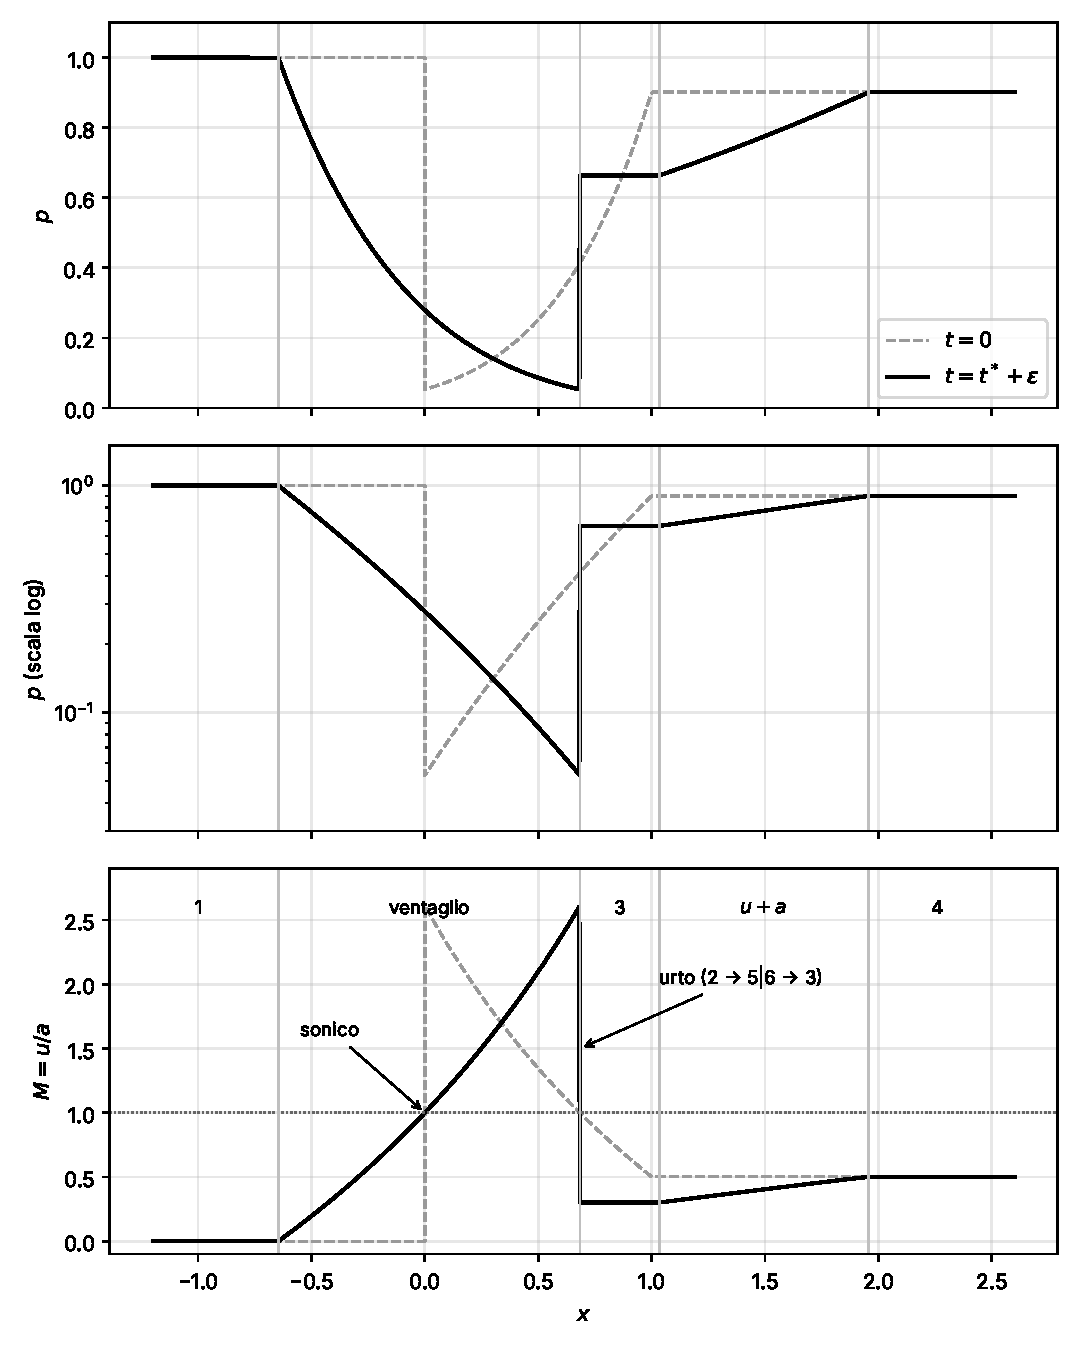
\includegraphics[width=0.8\textwidth]{profili_tstar.pdf}
  \caption{$p(x)$ in scala lineare e logaritmica e $M(x)$ a $t=0$ (tratteggio) e a $t=t^*+\varepsilon$.}
  \label{fig:profili}
\end{figure}
Fig.~\ref{fig:profili}, risposta alla richiesta principale. A $t^*+\varepsilon$ il ventaglio ha portato la
pressione da 1 a \num{0.053} con andamento continuo e Mach da 0 a \num{2.61}, passando per $M=1$ in $x=0$; la
compressione, che a $t=0$ occupava $0<x<1$, si è ridotta al salto verticale in $x^*$, dove $p$ risale di un
ordine di grandezza e $M$ crolla a \num{0.3}. A destra il plateau 3 e la rampa dell'onda $\upa$ fino allo stato
4. La pressione copre più di un ordine di grandezza: la scala lineare mostra il peso relativo dei salti, quella
logaritmica rende leggibile la parte bassa del ventaglio e l'entità del salto in $x^*$ (oltre un fattore 10).

\begin{figure}[H]
  \centering
  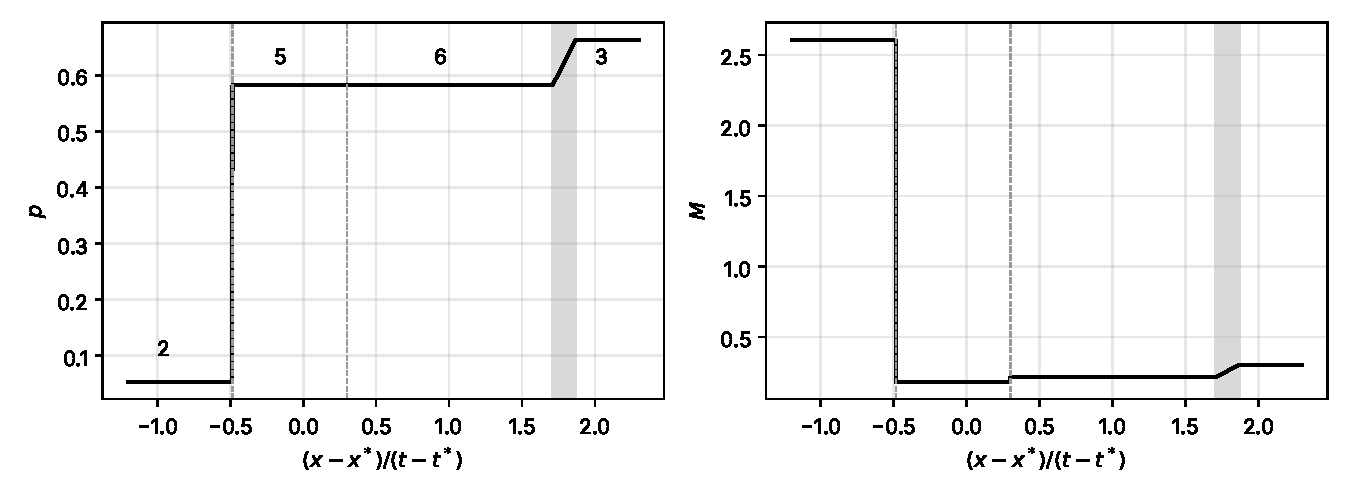
\includegraphics[width=0.95\textwidth]{struttura_salto.pdf}
  \caption{Struttura interna del salto in $x^*$ nella variabile $(x-x^*)/(t-t^*)$: urto, contatto
  (tratteggi) ed espansione $\upa$ (fascia grigia).}
  \label{fig:salto}
\end{figure}
Fig.~\ref{fig:salto}: il salto di fig.~\ref{fig:profili} ingrandito. L'urto porta $p$ da \num{0.053} a
\num{0.582}; il contatto non cambia $p$ ma cambia $M$ (da \num{0.180} a \num{0.213}), perché lo stato 5,
riscaldato dall'urto, ha velocità del suono maggiore; l'espansione $\upa$ completa il passaggio a 3.

\begin{figure}[H]
  \centering
  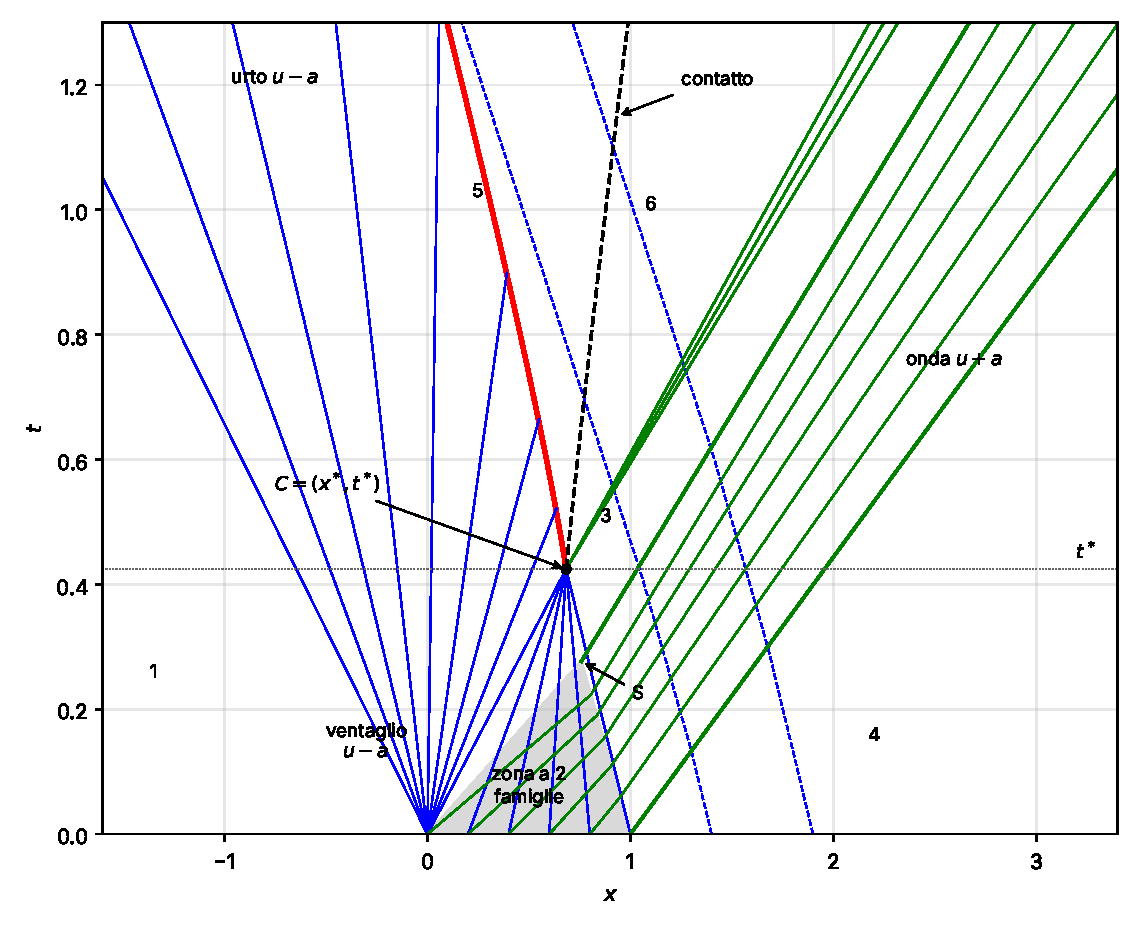
\includegraphics[width=0.85\textwidth]{xt.pdf}
  \caption{Piano $x$--$t$: $\uma$ in blu, $\upa$ in verde, urto in rosso, contatto tratteggiato; in grigio la zona
  a due famiglie. Dopo $t^*$ urto e contatto sono qualitativi.}
  \label{fig:xt}
\end{figure}
Fig.~\ref{fig:xt}: il ventaglio centrato nell'origine e la compressione convergente nel centro $C$, con la coda
del ventaglio che coincide con la prima $\uma$ della compressione. Le $\upa$ uscenti dal tratto lineare, piegate
nella zona d'interazione, ne escono divergenti (espansione). Da $C$ partono l'urto, che piega verso sinistra
entrando nel ventaglio e tende alla pendenza $u_\infty-a_\infty$, il contatto, che tende alla velocità
$u_\infty$, e la stretta espansione $\upa$ fra 6 e 3. Le $\uma$ che vengono dallo stato 4 (tratteggiate)
attraversano l'onda $\upa$ e lo stato 3 e raggiungeranno anch'esse l'urto, da valle.

\begin{figure}[H]
  \centering
  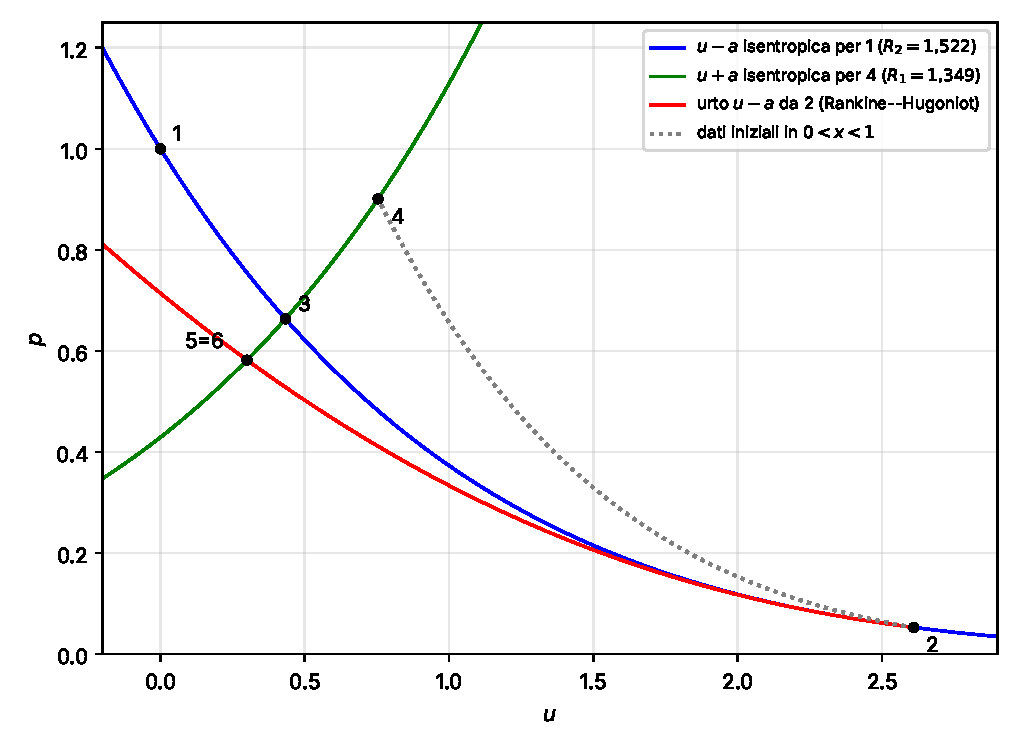
\includegraphics[width=0.66\textwidth]{pu_lin.pdf}\\
  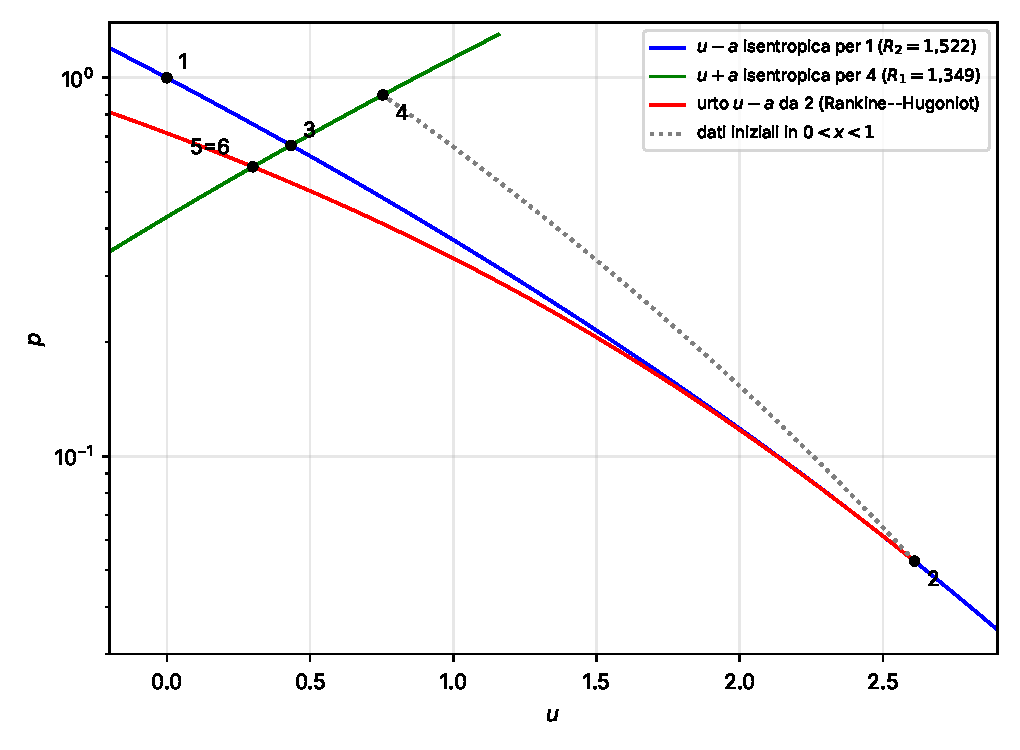
\includegraphics[width=0.66\textwidth]{pu_log.pdf}
  \caption{Piano $p$--$u$, scala lineare (sopra) e logaritmica (sotto).}
  \label{fig:pu}
\end{figure}
Fig.~\ref{fig:pu}. Gli stati 1, 2 e 3 stanno sulla stessa isentropica $\uma$ ($R_2=\num{1.522}$): il ventaglio
porta da 1 a 2, la compressione riporterebbe da 2 a 3 lungo la stessa curva. Gli stati 3 e 4 stanno
sull'isentropica $\upa$ di 4. I dati iniziali del tratto lineare (punteggiato) non stanno su nessuna delle due
curve: è il segno che sono presenti entrambe le famiglie. In $C$ la curva di Rankine--Hugoniot da 2 sta sotto
l'isentropica e taglia l'isentropica $\upa$ in $5=6$, a velocità e pressione minori di 3: per questo dietro
l'urto serve un'espansione. Il contatto non si vede (5 e 6 coincidono, ma con impedenze $\rho a$ diverse,
\num{0.49} e \num{0.58}). Lo stato asintotico è l'intersezione delle isentropiche di 1 e di 4, cioè 3. La scala
lineare mostra bene la zona di $C$; quella logaritmica rende leggibile la regione di bassa pressione vicino a 2,
dove la curva di Rankine--Hugoniot e l'isentropica partono tangenti (stessa tangente e curvatura) e si separano
solo per salti forti.

%==============================================================================
\section{Discussione fisica}
\textbf{Istante di formazione.} Il tratto lineare non è un'onda semplice ($R_2$ varia di circa l'8\%): nella
breve zona d'interazione le $\uma$ si piegano un po' verso sinistra (da $u_4-a_4=-\num{0.75}$ a
$u_3-a_3=-\num{1.00}$ quella da $x=1$). Con le pendenze dopo la separazione, $u-a=2R_{2,1}-3R_1(x_0)$, il
gradiente sarebbe \num{2.61} e $t\approx\num{0.38}$: l'urto nasce un po' prima di $t^*$ e la coalescenza non è
esattamente in un punto. La struttura (urto forte nato quasi tutto insieme, contatto, espansione $\upa$) non
cambia; uso l'istante della traccia.

\textbf{Perché nasce un urto forte.} La corrente supersonica a $M=\num{2.61}$ della coda del ventaglio va a
sbattere contro il gas lento dello stato 3, come contro un pistone: la compressione centrata non ha il tempo di
formare l'urto per gradi, che nasce già con $\Ms\approx3$. A questa intensità l'approssimazione isentropica
dell'urto (lecita per $\Ms\lesssim\num{1.2}$) non vale: darebbe direttamente lo stato 3, mentre le
Rankine--Hugoniot danno $p^*=\num{0.582}$ e un'espansione $\upa$ non trascurabile. L'entropia prodotta
($s_5/s_2=\num{1.61}$) resta nelle particelle urtate, che si comportano come una bolla calda.

\textbf{Evoluzione e regime asintotico.} L'espansione ``vive per sempre'', la compressione degenera: l'urto viaggia
a $W<0$ dentro un ventaglio le cui $\uma$ (più veloci) lo raggiungono da monte, quindi vede a monte gas sempre più
lento e caldo e si indebolisce. Alla fine la parte supersonica del ventaglio è stata assorbita: l'espansione
asintotica verso sinistra è subsonica (coda a $M=\num{0.30}$) e il salto netto fra 1 e 4 è una doppia
espansione con lo stato centrale 3. Il regime asintotico è un pseudo-Riemann: ne dà gli stati, non i tempi
dell'interazione urto--ventaglio, che si potrebbe seguire solo con le caratteristiche e le relazioni d'urto
punto per punto.
\end{document}
